%Tu si môžete zaznačiť, že pracujete na danej veci. V prípade, že ste napísali len časť a ďalej už
%nechcete, alebo ste hotoví tak sa odtiaľ odpíšte. Bolo by však fajn, aby jedu vec robil jeden
%človek ak celok a zvyšný len kontrolovali
%vypracuva: Zaba 
\input include/include.tex

\begin{document}

\velkynadpis{Ťahák 1}

Python je interpretovaný programovací jazyk. To znamená, že ho netreba kompilovať a príkazy vykonáva priamo za behu.
Preto vieme veľmi jednoduchým spôsobom skúšať jednoduché príkazy bez toho, aby sme potrebovali zložitú štruktúru.
Môžeme teda Python použiť ako jednoduchú kalkulačku.

\lstlang{python}\begin{lstlisting}
>>> 5
5
>>> 10+2*3
16
>>> 10/3
3
>>>10/3.0
3.333333333
>>> 3**4
81
\end{lstlisting}

Videli sme, že keď mu dáme nejaký matematický výraz (dve hviezdičky predstavujú umocňovanie), tak nám ho
vyhodnotí a vypíše výsledok.

\nadpis{Premenné}

Premenná je krabička (miesto v pamäti), kam si program ukladá dáta. Každá premenná má svoje \texttt{meno} (jednoznačný
identifikátor), ktorým sa na konkrétnu premennú odkazujeme inde v programe. Keď v programe použijeme meno nejakej premennej
máme na mysli hodnotu, ktorá je v nej uložená. To nám umožňuje vytvárať výrazy obsahujúce premenné.

Najčastejšie si pamätáme čísla alebo reťazce písmen (stringy). Obsah stringu sa obaľuje úvodzovkami, aby sme ich vedeli rozlíšiť
od premenných. Do premennej zapisujeme hodnotu pomocou znaku \texttt{=}.

\lstlang{python}\begin{lstlisting}
>>> a = 5
>>> a
5
>>> a+6
11
>>> b = "ahoj"
>>> b
'ahoj'
\end{lstlisting}

No a samozrejme premenné môžeme aj kombinovať, vkladať hodnotu jednej premennej do druhej, poprípade porovnávať ich obsah.
Porovnávame pomocou \textbf{dvoch} rovná sa \texttt{==} a výsledok tejto operácie je jedna z dvoch logických hodnôt \texttt{True}
a \texttt{False}.

\lstlang{python}\begin{lstlisting}
>>> a=5
>>> b=4
>>> b
4
>>> b=a
>>> b
5
>>> a==b
True
>>> a==4
False
\end{lstlisting}

Naviac sa nám zíde vedieť zmeniť číslo na string a opačne. Na to slúžia funkcie \texttt{str()} a \texttt{int()}.

\lstlang{python}\begin{lstlisting}
>>> a=4
>>> str(a) + "hoj"
'4hoj'
>>> b="14"
>>> int(b) + 5
19
\end{lstlisting}

\nadpis{Kreslenie}

Keď už chceme robiť nejaké tie hry, asi by bolo fajn, aby sme vedeli niečo kresliť. Či už pozadie, bojovníkov, plávajúcu ryby \dots
Na začiatok si ukážeme to najjednoduchšie: kreslenie pozadia.

\texttt{Poznámka: } Kreslenie hocičoho ďalšieho bude rovnako jednoduché, nebojte sa. Jediný rozdiel bude v tom ako použijeme \texttt{kreslic}.
Niektoré z nasledujúcich informácií teda budú mierne nepresné alebo dokonca nesprávne, aby sme to mali jednoduchšie. Ich opravenie však bude
jednoduché trochu neskôr.

\nadpis{Kreslic}

Vždy keď chceme niečo nakresliť na plochu, musíme o to poprosiť \texttt{kreslic}. To je totiž naša jediná možnosť vykresľovania. Preto treba vedieť
ako správne poprosiť kreslic, aby niečo spravil.

\begin{itemize}
	\item \texttt{kreslic.obdlznik((x,y),sirka,vyska,okraj)} -- bod $(x,y)$ hovorí, kde sa má nachádzať ľavý horný okraj obdĺžnika. $sirka$ a $vyska$
		určuje, aký je obdĺžnik veľký. No a premenná $okraj$ hovorí, aký hrubá je čiara, ktorá vykreslí tento obdĺžnik. Ak tento parameter
		vynecháte (naozaj tam nič nedáte) obdĺžnik bude vyplnený.
	\item \texttt{kreslic.elipsa((x,y),sirka,vyska,okraj)} -- toto sa až podozrivo podobá na obdĺžnik. A veru tomu tak aj je. Akurát namiesto obdĺžnika
		sa nakreslí elipsa, ktorá je do tohoto obdĺžnika vpísaná (takže sa dotýka všetkých jeho stien). Ak teda chceme nakresliť kruh, musí
		byť nás opísaný obdĺžnik štvorec, $sirka == vyska$.
	\item \texttt{kreslic.ciara((x1,y1),(x2,y2),hrubka)} -- nakreslí sa čiara od bodu $(x1,y1)$ do bodu $(x2,y2)$ s hrúbkou $hrubka$.
	\item \texttt{kreslic.mnohouholnik([(x1,y1),(x2,y2),\dots],okraj)} -- nakreslí mnohouholník, ktorého vrcholy sú v bodoch $(x1,y1)$, $(x2,y2)$ \dots
\end{itemize}

\nadpis{Súradnice}

Celý čas sme si vraveli, že sa to vykreslí na nejakú pozíciu. Kde však táto pozícia je? Kde sa napríklad nachádza bod $(50,100)$? Na to treba vedieť,
ako fungujú súradnice v našom okne. Naše okno je široké $okno.sirka$ a vysoké $okno.vyska$. Toto sú dve premenné, ktoré hovoria o tom, ako veľké dané
okno je. Naviac ľavý horný roh má súradnicu $(0,0)$ a pravý dolný roh má súradnicu $(okno.sirka,okno.vyska)$. Zvyšné súradnice sú rozmiestnené
rovnomerne medzitým.

Uvedomte si, že smerom nadol \textbf{stúpa} $y$-ová súradnica a doprava \textbf{stúpa} $x$-ová súradnica.

\nadpis{Farba}

A aby naše obrázky neboli také nudné, bolo by dobré vedieť zmeniť farbu, ktorou kreslíme. Na to musíme povedať \texttt{kreslic}, akú farbu má používať.
To vieme tak, že zmeníme premennú $kreslic.farba$. Tej buď priradíme nejakú známu farbu ako je $Farba.MODRA$, $Farba.ZLTA$ alebo si namiešame vlastnú farbu
$Farba(cervena, zelena, modra)$, kde $cervena$, $zelena$ a $modra$ sú čísla od $0$ po $255$, ktoré udávajú množstvo danej farby vo výsledku.

Zoznam dostupných farieb: $Farba.CIERNA$, $Farba.BIELA$, $Farba.MODRA$, $Farba.ZELENA$, $Farba.CERVENA$ a $Farba.ZLTA$.

\bigskip

Na nasledujúcom príklade si môžete pozrieť, ako by vyzeralo jednoduché vykreslenie štyroch útvarov
do okna s veľkosťou $600$ krát $400$.

\lstlang{python}\begin{lstlisting}
kreslic.farba = Farba.CERVENA
kreslic.obdlznik((0,0),200,80,5)
kreslic.farba = Farba(0,255,0)
kreslic.elipsa((300,200),100,100)
kreslic.farba = Farba.MODRA
kreslic.ciara((500,300),(okno.sirka,okno.vyska),5)
kreslic.mnohouholnik([(0,100),(100,100),(50,200)])
\end{lstlisting}

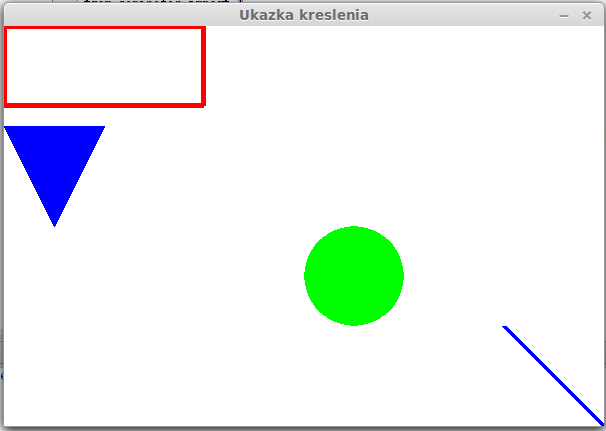
\includegraphics[scale = 0.5]{priklad1.png}

\end{document}
